\chapter{Other Experiments}\label{chp:LABEL_CHP_5}

Building upon the concepts and techniques discussed throughout this work, it is already possible to create a variety of compelling raymarched scenes. This chapter is dedicated to showcasing several images produced during the development of this research, employing the methods previously presented.

\section{Examples of Rendered Scenes}

Furthermore, as mentioned before, Ray Marching is largely used for the rendering of fractals, from a simpler (Sierpinsky Triangle), to more generalized ones, such as Kaleidoscopic IFSs (Iterated Function Systems), as displayed in Figure \ref{fig:fractals}.

The technique used to render the Sierpinsky Triangle is just a variation of domain repetition, applied to tetrahedrons. As discussed, this means the additional cost for calculating and comparing infinite distances is reduced to just one repeating object. In fact, this process can be generalized to all platonic objects, not only tetrahedrons, and with clever space folding and rotations, a 2010 user of Fractal Forums \cite{Godar2022KaleidoscopicIFSFractals} came up with what they called Kaleidoscopic IFS, a now mainstay on the Fractal Rendering Community.

\begin{figure}[ht]
    \centering
    \begin{minipage}{0.45\textwidth}
        \centering
        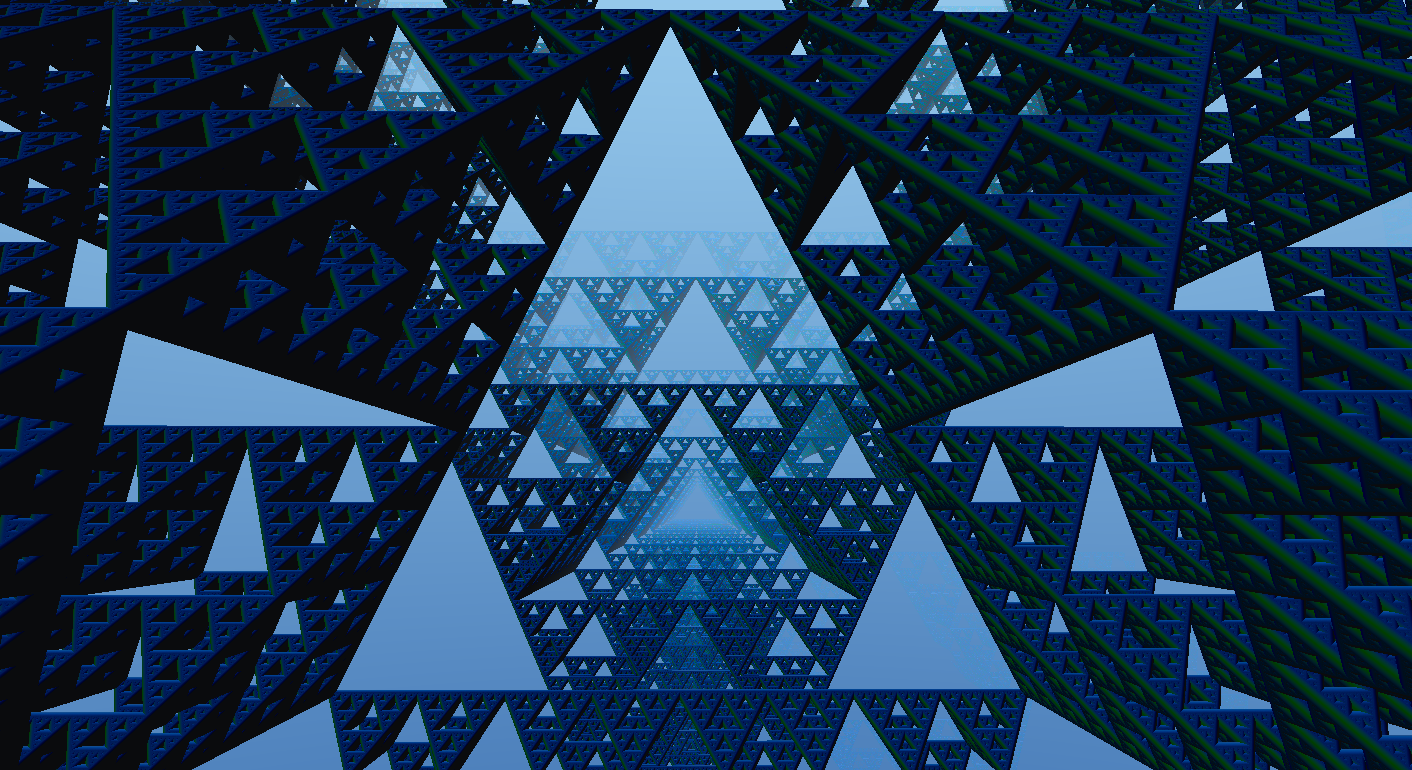
\includegraphics[width=\linewidth]{imagens/fract1.png}\\
        Sierpinsky Triangle
    \end{minipage}%
    \hfill
    \begin{minipage}{0.45\textwidth}
        \centering
        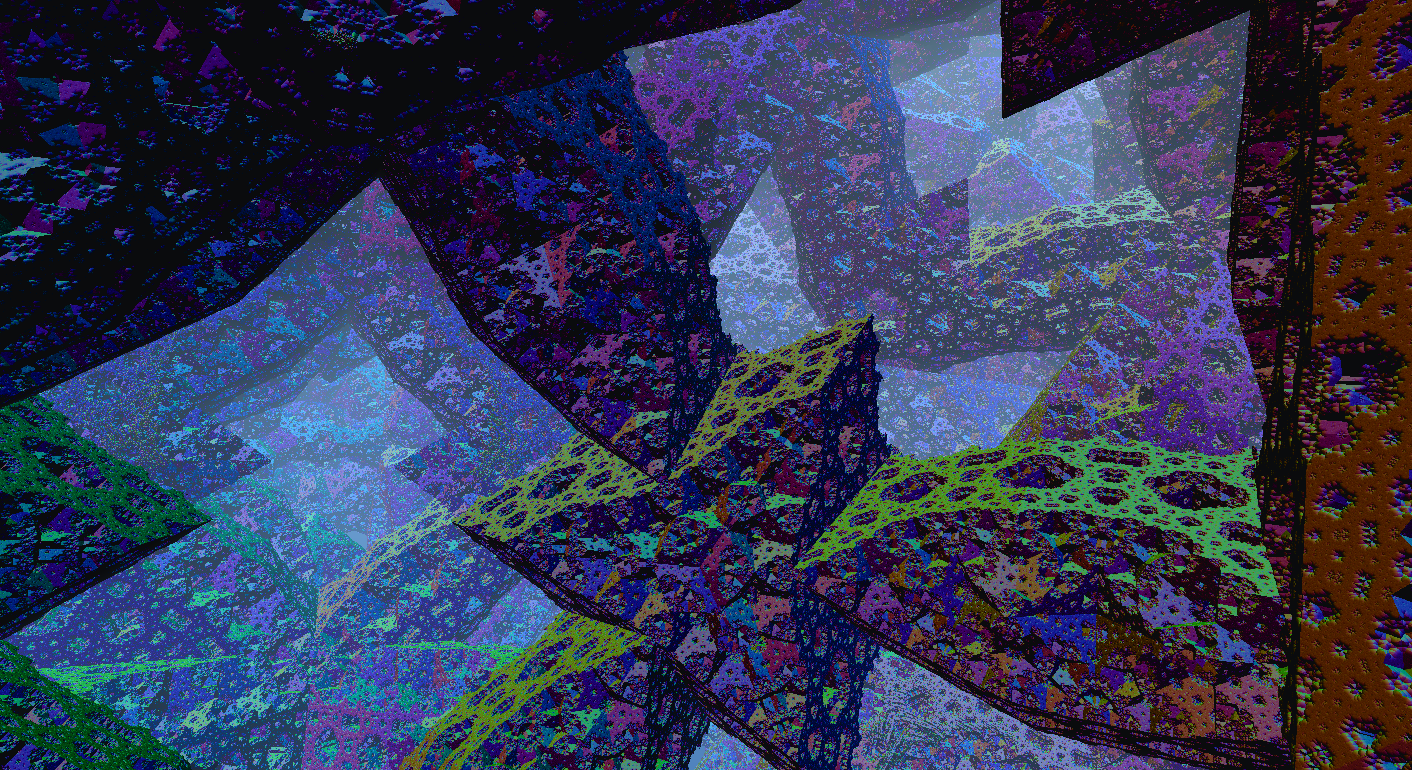
\includegraphics[width=\linewidth]{imagens/fract2.png}\\
        Hollow Insides of a Kaleidoscopic IFS
    \end{minipage}

    \vspace{1em} % space between rows
    % Row 1
    \begin{minipage}{0.45\textwidth}
        \centering
        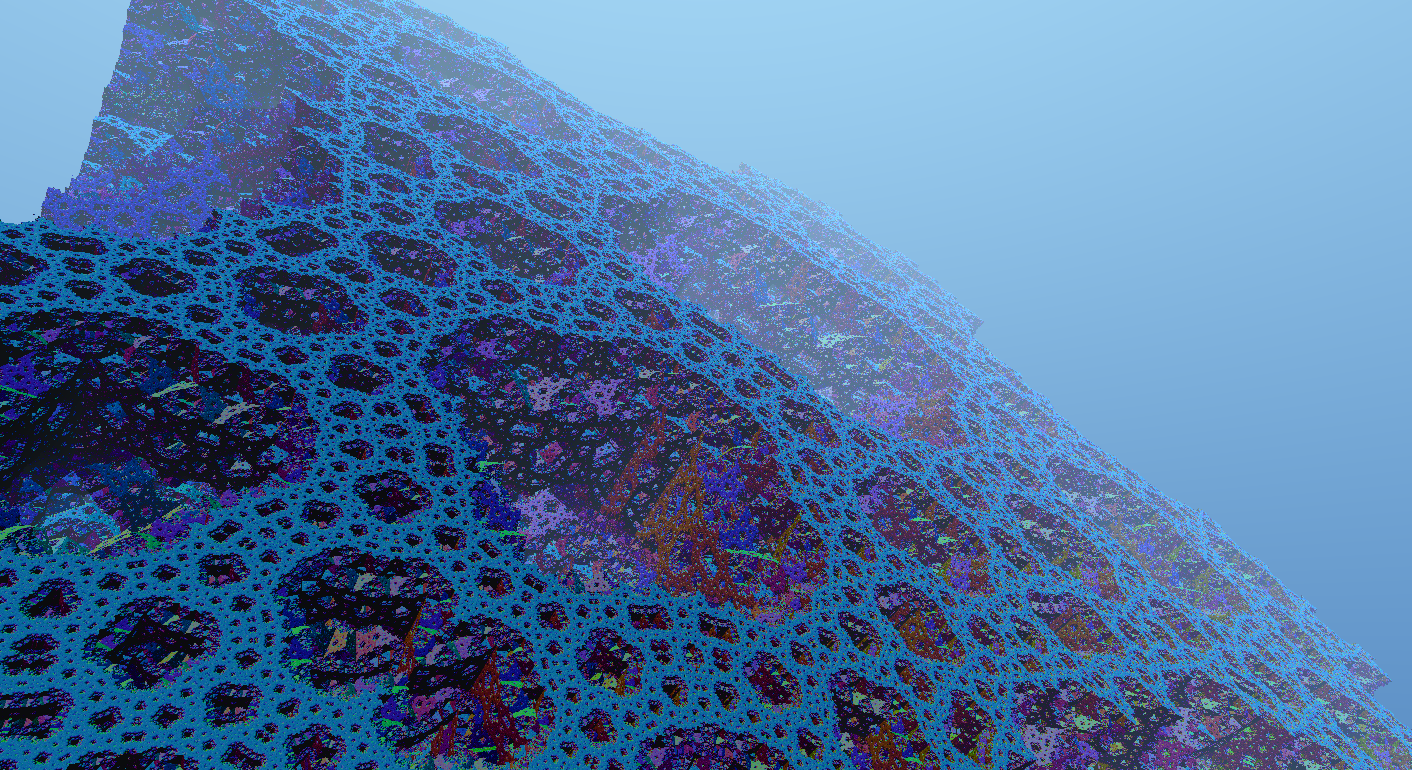
\includegraphics[width=\linewidth]{imagens/fract3.png}\\
        Outside of Kaleidoscopic IFSs
    \end{minipage}%
    \hfill
    \begin{minipage}{0.45\textwidth}
        \centering
        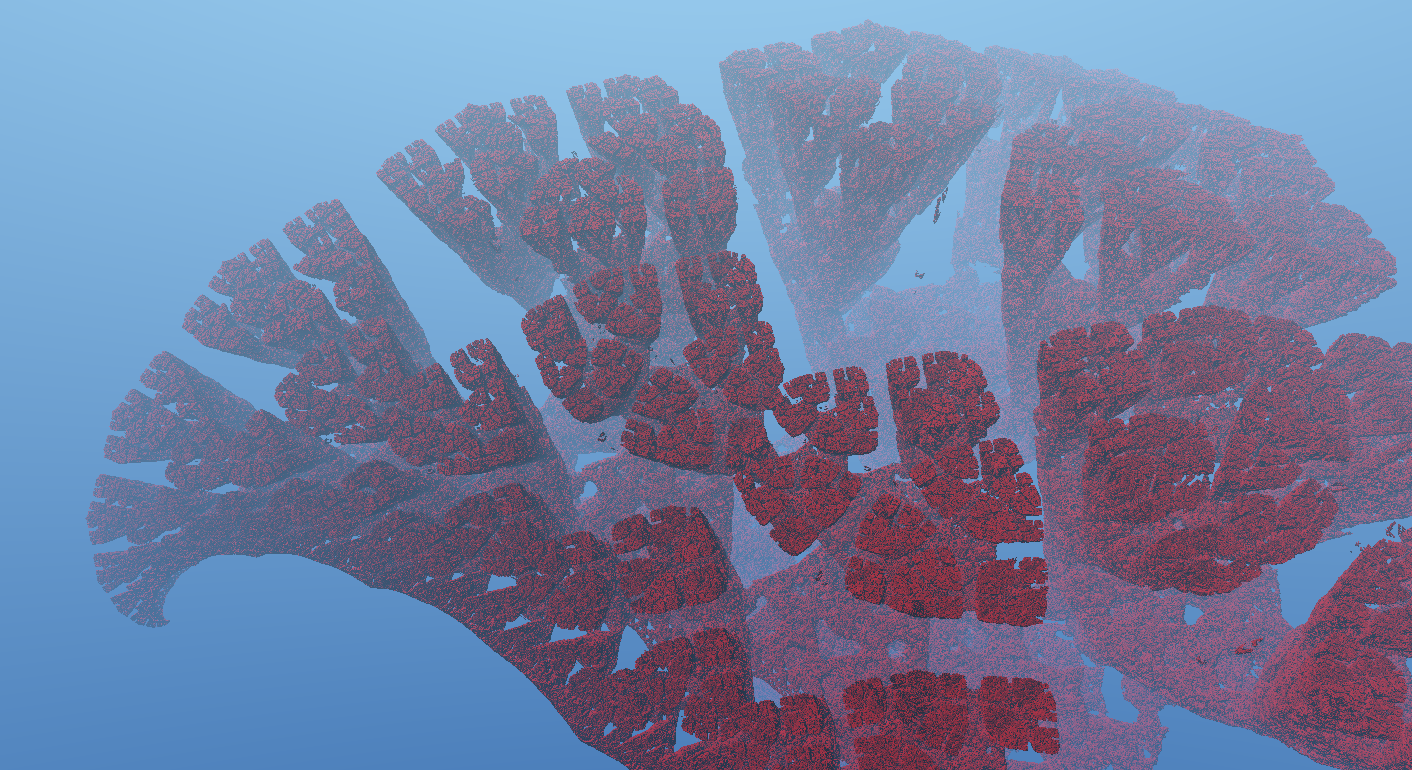
\includegraphics[width=\linewidth]{imagens/fract4.png}\\
        Outside of Kaleidoscopic IFSs
    \end{minipage}

    \vspace{1em} % space between rows

    % Row 2
    \begin{minipage}{0.45\textwidth}
        \centering
        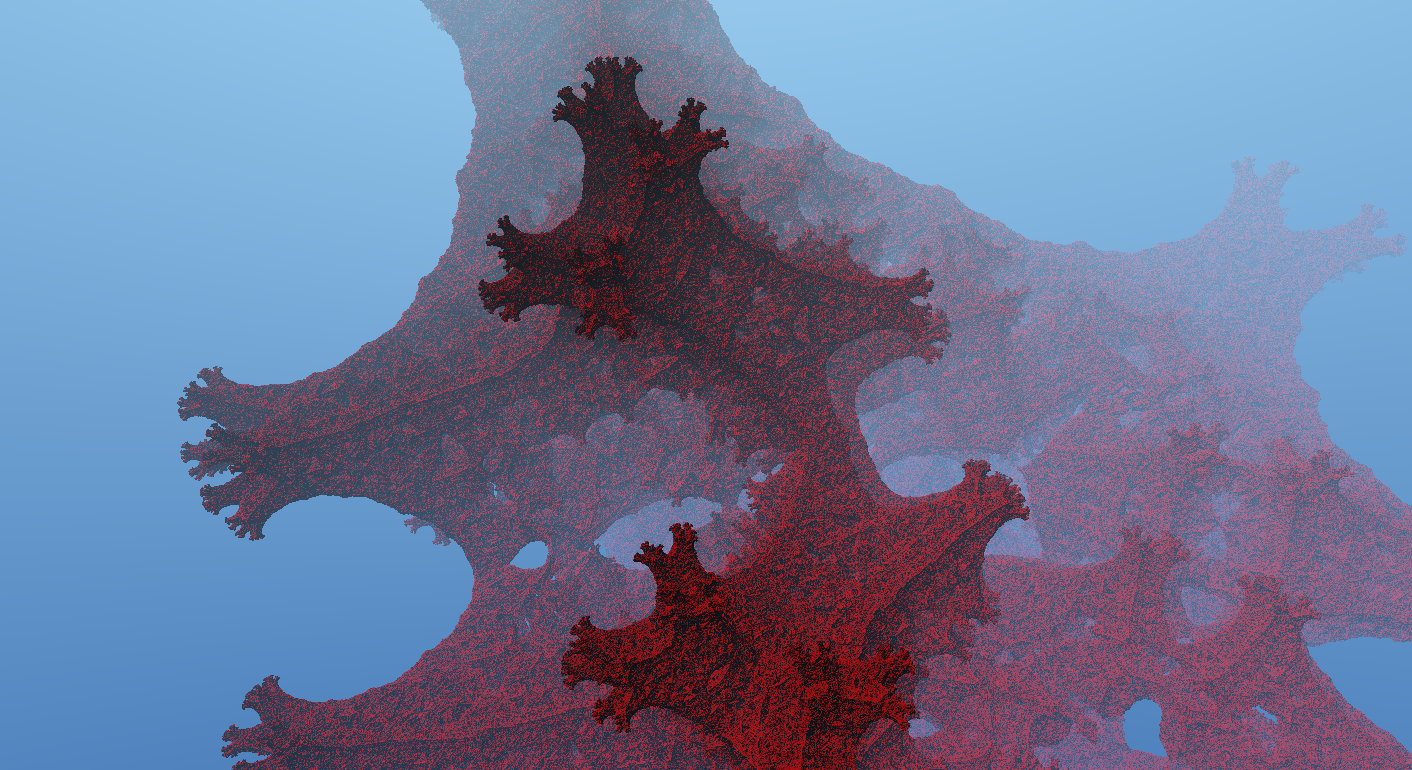
\includegraphics[width=\linewidth]{imagens/fract5.png}\\
        Outside of Kaleidoscopic IFSs
    \end{minipage}%
    \hfill
    \begin{minipage}{0.45\textwidth}
        \centering
        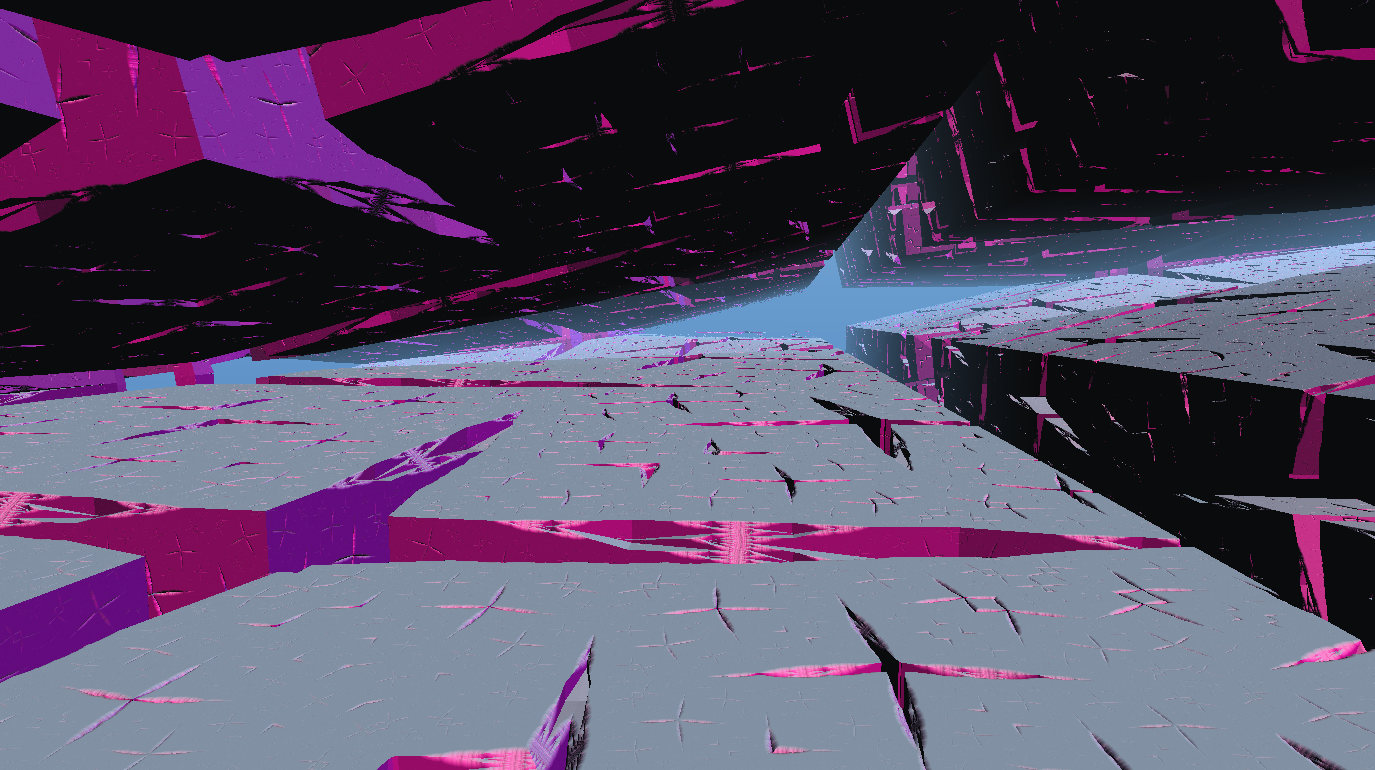
\includegraphics[width=\linewidth]{imagens/fract6.png}\\
        Insides of Kaleidoscopic IFS
    \end{minipage}

    % Row 3
    \begin{minipage}{0.45\textwidth}
        \centering
        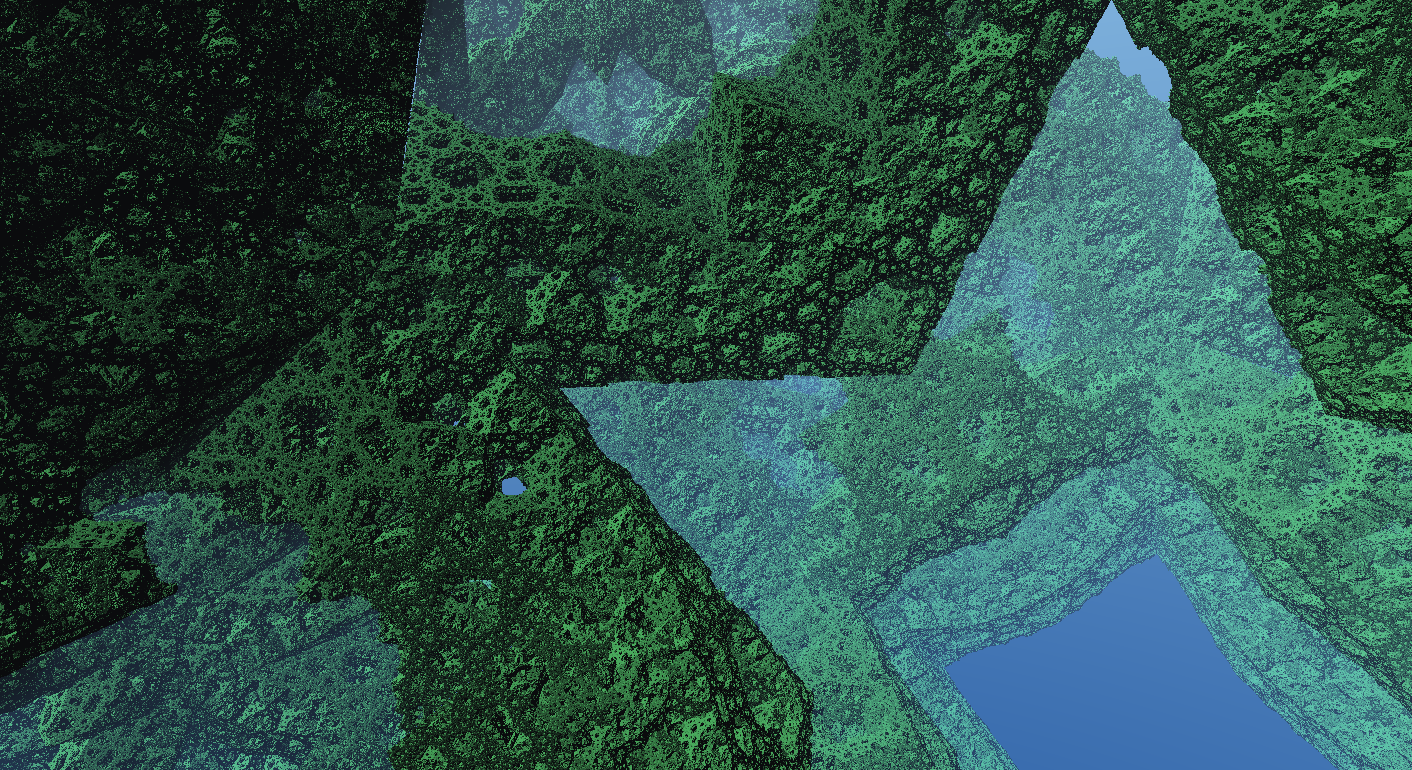
\includegraphics[width=\linewidth]{imagens/fract7.png}\\
        Insides of Kaleidoscopic IFS
    \end{minipage}%
    \hfill
    \begin{minipage}{0.45\textwidth}
        \centering
        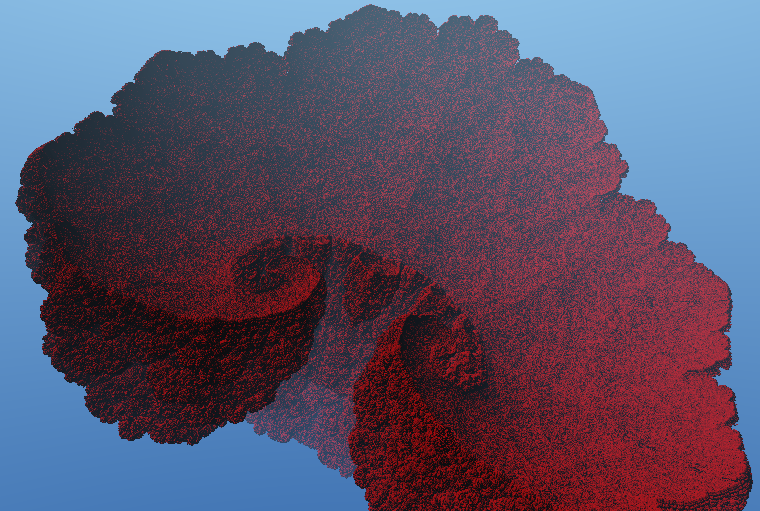
\includegraphics[width=\linewidth]{imagens/fract8.png}\\
        Outside of Kaleidoscopic IFSs
    \end{minipage}

    \caption{Multiple fractals using the Kaleidoscopic IFS technique.}
    \label{fig:fractals}
    
\end{figure}


